\clearpage
\begin{figure}[p]
\centering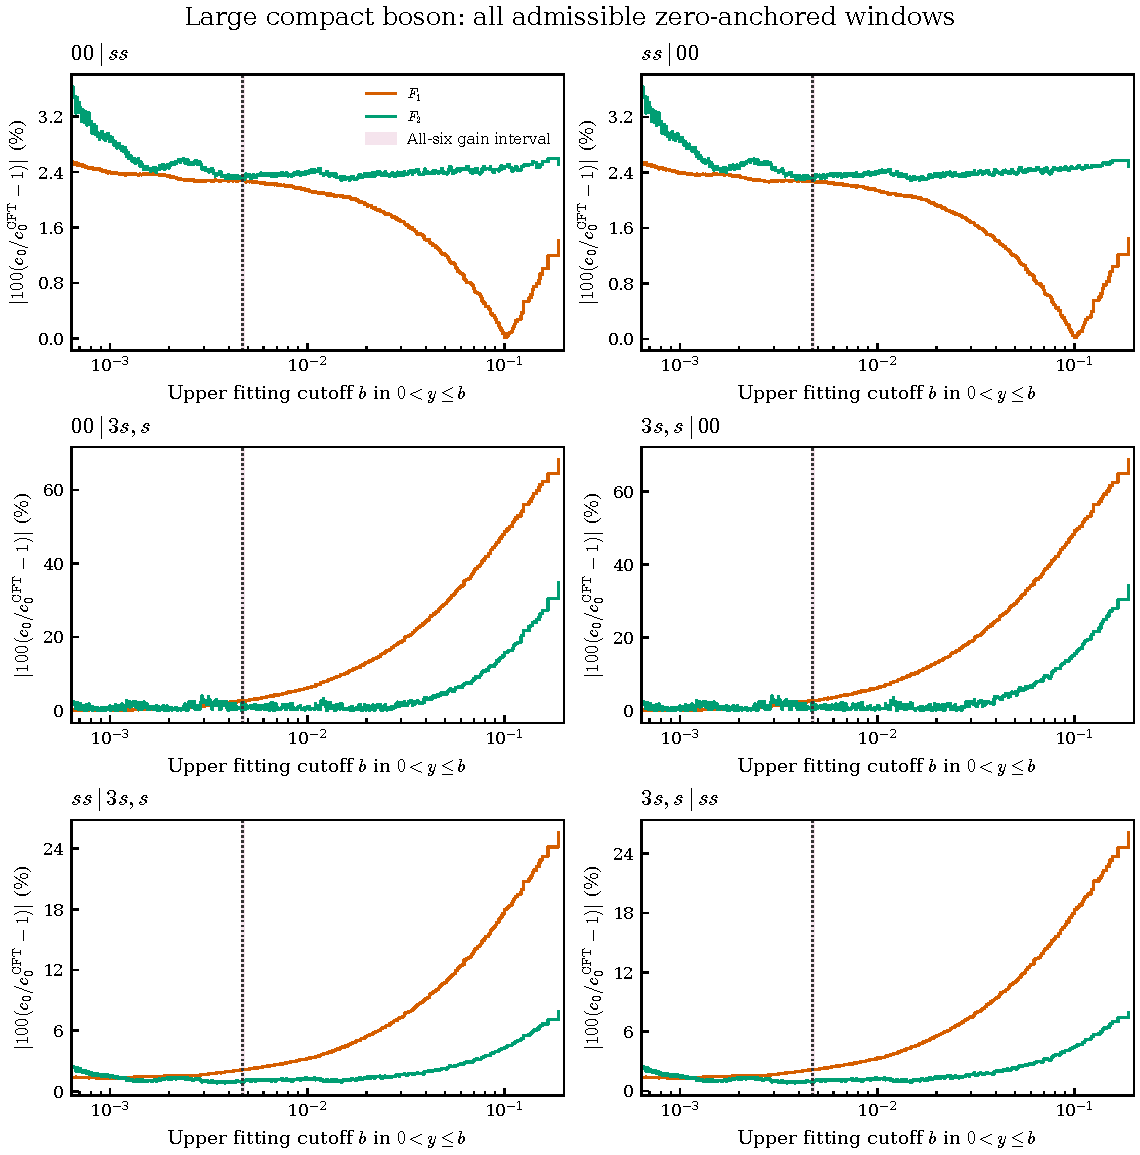
\includegraphics[width=\textwidth,height=.83\textheight,keepaspectratio]{../figs/zero_anchored_cutoff_scan.pdf}
\caption{Large-boson leading-coefficient accuracy across all admissible zero-anchored windows $W_y=(0,v]$ through $v=0.20$, using $p=1/2$ and $\ell=6,7,8,9,10$. The plotting symbol $b$ on the horizontal axis denotes the trial upper cutoff $v$, not a primary-state label. Each step corresponds to a distinct selected data set with at least forty training observations after any chain-size omission. Both powers of $F_2$ are fixed to Table~\ref{tab:complement-theory}; $F_1$ uses only its leading power. The ordinate is $|\eta_c|$ from Eq.~\eqref{eq:metrics}, on a linear scale. The dotted line marks the previous candidate $v=0.0047$, and the shaded band marks Eq.~\eqref{eq:zero-equivalent-cutoffs}. The current prescribed cutoff is $0.005$; its counts and minimum training sizes are in Table~\ref{tab:common-window-counts}.}
\label{fig:zero-anchored-scan}
\end{figure}
\clearpage
\begin{figure}[p]
\centering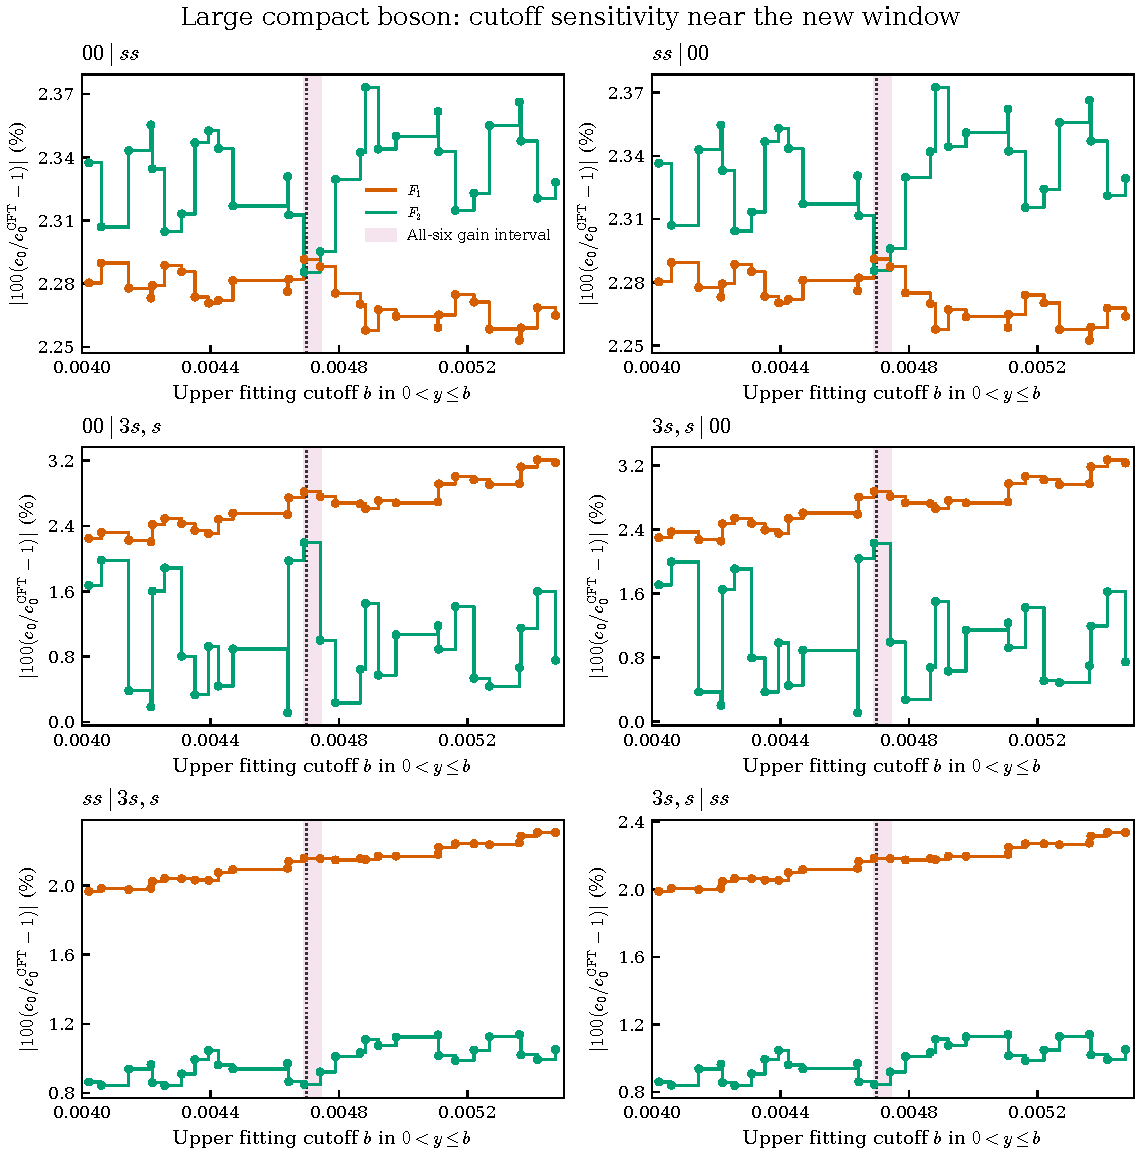
\includegraphics[width=\textwidth,height=.83\textheight,keepaspectratio]{../figs/zero_anchored_cutoff_zoom.pdf}
\caption{Historical cutoff sensitivity around the previous large-boson candidate $0.0047$, using the same data, models and discrepancy as Fig.~\ref{fig:zero-anchored-scan}. Markers show actual changes of data membership; both axes are linear. The shaded historical interval has 311 points per direction from 68 chain sizes. The nearest selections outside it lose the all-six leading-coefficient gain, as quantified in Table~\ref{tab:common-window-neighbors}. The residual reduction alone does not establish coefficient recovery.}
\label{fig:zero-anchored-zoom}
\end{figure}
\clearpage
